\documentclass[notitlepage]{report}
\usepackage{graphicx}
\usepackage{amsmath}
\usepackage{amssymb}
\usepackage[parfill]{parskip}
\newcommand\numberthis{\addtocounter{equation}{1}\tag{\theequation}}


\usepackage{titling}

\title{Desmos Polygonal Number Diagrams (draft)}
\author{Dan MacKinnon}

\begin{document}
\maketitle
\begin{abstract}
\noindent
Polygonal numbers, like the triangular, square, and pentagonal numbers, are closely identified with (or even defined in terms of) the diagrams that they are associated with. The functional programming capabilities of the Desmos graphing calculator provides fun and interesting ways of exploring number diagrams like those associated with polygonal numbers. This short article provides one approach that can be used to build polygonal number diagrams in Desmos.  
\end{abstract}

\section*{Polygonal numbers}
For a given $k \in \mathbb{Z}^+, k>2$, the $k$-polygonal numbers are a recursively defined integer sequence, as shown in Equation (\ref{eq:defn1}). 

\begin{align*}
    p_{k, 1} &= 1 \\
    p_{k,i} &= p_{k,i-1} + (k-2)i - (k-3)
    \numberthis
    \label{eq:defn1}
\end{align*}

For a term in the sequence $n = p_{k,i}$, $n$ dots can be arranged in a regular $k$-polygon built up of $i$ layers (traditionally referred to as \textit{gnomons}), as shown for the pentagonal numbers ($k=5$) of Figure (\ref{fig:pentagonals}). 

\begin{figure}[!htb]
    \centering
    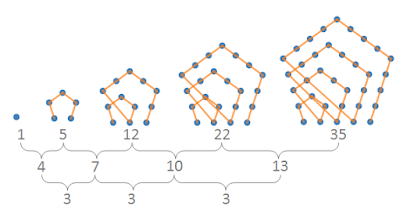
\includegraphics[width=0.5\linewidth]{pentagonal_numbers.PNG}
    \caption{The first few pentagonal numbers, showing first and second differences}
    \label{fig:pentagonals}
\end{figure}

If $n$ is the $i$th $k$-polygonal number, it can be drawn as a layered regular $k$-polygon with $i$ gnomon layers, as shown for the third pentagonal number $12$, $p_{5,3}=12$, in Figure (\ref{fig:gnomons}.

\begin{figure}[!htb]
    \centering
    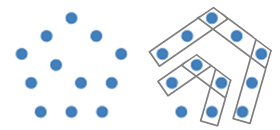
\includegraphics[width=0.5\linewidth]{pentagon_with_gnomon.PNG}
    \caption{Pentagonal number diagram $n=12$ with gnomons}
    \label{fig:gnomons}
\end{figure}

\section*{Placing any $n$ in a $k$-polygonal diagram}

Let $n,k \in \mathbb{Z}^{+}$, $k > 2$. We would like to draw the $k-$polygonal number diagram ``up to'' $n$. If $n$ happens to actually be a $k-$polygonal number, this will be a complete diagram with $n$ dots in a layered $k$-polygon. Otherwise, this will be a diagram whose outer gnomon layer is incomplete.

Figure (\ref{fig:hexagonals}) shows hexagonal number ($k = 6$) diagrams for the numbers 15 and 26. Because 15 actually is a hexagonal number, the diagram is complete. The diagram for 26 shows an incomplete diagram, with an incomplete outer layer.

\begin{figure}[!htb]
    \centering
    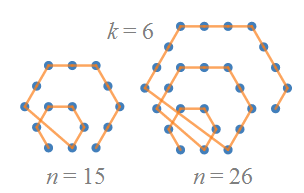
\includegraphics[width=0.5\linewidth]{hexagonal_and_no.PNG}
    \caption{Two hexagonal diagrams ($k = 6$), 15 is hexagonal, 26 is not}
    \label{fig:hexagonals}
\end{figure}


\subsection*{Finding the gnomon for $n$ and $k$}

The recursive definition for $p_{k,1}$ in Equation (\ref{eq:defn1} yields formulas stated as a summation (\ref{eq:summation}) and a direct calculation (\ref{eq:quad}).

\begin{equation}
    p_{k,i} = \sum^{i}_{j=1}\left[(k-2)j-(k-3)\right]
    \label{eq:summation}
\end{equation}

\begin{equation}
    p_{k,i} = \frac{(k-2)i(i+1)}{2} - (k-3)i
    \label{eq:quad}
\end{equation}

Applying the quadratic formula to solve $n-p_{k,i}=0$ provides us with

\begin{equation}
    g\left(n,k\right)=\frac{\left(k-4\right)+\sqrt{\left(k-4\right)^{2}+8n\left(k-2\right)}}{2\left(k-2\right)}
     \label{eq:quadform}
\end{equation}

This allows us to identify the gnomon layer $\text{gnomon}(n,k)$ that a given $n$ will sit in within a $k$-polygonal diagram (\ref{eq:gnomon}).

\begin{equation}
    \text{gnomon}\left(n,k\right) = \text{floor}\left(g\left(n\right)\right)  
    \label{eq:gnomon}
\end{equation}

\subsection*{The position of $n$ within its gnomon layer}

The size of the gnomon layer that $n$ will sit in (how many dots would be in the layer within the diagram) is given by Equation (\ref{eq:gnomon-size}).

\begin{equation}
\text{gsize}\left(n,k\right)= 1+(\text{gnomon}\left(n,k\right)-1)\cdot\left(k-2\right)
\label{eq:gnomon-size}
\end{equation}

To find the position of the $n$th dot within the gnomon, we need to count the number of dots that came before it within that gnomon. To do this we can sum up to $n-1$ over a function whose value is $0$ for all $i$ where $gnomon(i,k)<gnomon(n,k)$, and whose value is $1$ for those $i$ where $gnomon(i,k)=gnomon(n,k)$. This sum that gives us the "depth" of \textit{n} within its gnomon is provided by Equation (\ref{eq:gnomon-depth}).

\begin{equation}
    \text{gdepth}\left(n,k\right)=\sum_{i=1}^{n}\left(\text{floor}\left(\frac{gnomon\left(i,k\right)}{gnomon\left(n,k\right)}\right)\right)
    \label{eq:gnomon-depth}
\end{equation}

\section*{Drawing the diagram}

For a given $n,k \in \mathbb{Z}^{+}$, $k > 2$, the preceding sections tell us which gnomon $n$ will be placed in in a $k$-polygonal diagram, and in which spot along the gnomon. 

To complete the diagram, we need to also determine how much the gnomon is bent at the particular position that $n$ finds itself at. Because the gnomon is a layer in a regular $k$-gon, it bends in increments of the base angle $alpha$ that is given by Equation (\ref{eq:angle}).


\begin{equation}
    \alpha=\left(\pi-((k-2)*(\pi/k))\right)
\label{eq:angle}
\end{equation}

If we are at a position in some gnomon layer in a $k$-polygonal diagram, the bend at which we find $i$ is given by Equation (\ref{eq:bends}).

\begin{equation}
\text{bend}\left(n,k\right)=\sum_{i=1}^{\text{gdepth}\left(n\right)}\text{ceil}\left(\frac{i}{\text{gsize}\left(n\right)}\left(k-2\right)\right)
\label{eq:bends}
\end{equation}


\section*{leftovers}

\begin{equation}
x_{kn}\left(l\right)=-g_{nomon}\left(l\right)\cos\left(a_{ngle}\right)-\sum_{j=1}^{g_{depth}\left(l\right)}\cos\left(s_{k}\left(j,l\right)\cdot a_{ngle}\right)
\end{equation}

\begin{equation}    y_{kn}\left(l\right)=g_{nomon}\left(l\right)\sin\left(a_{ngle}\right)+\sum_{j=1}^{g_{depth}\left(l\right)}\sin\left(s_{k}\left(j,l\right)\cdot a_{ngle}\right)
\label{eq:yformula}
\end{equation}

The formulas for $x_{kn}$ and $y_{kn}$ express the idea of placing the point corresponding to the current polygonal number at the right spot in the correct gnomon layer for that number, as shown in Figure (\ref{fig:yannotated}).

% \begin{figure}
%     \centering
%     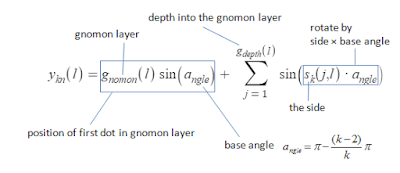
\includegraphics[width=0.5\linewidth]{annotated_eqn.PNG}
%     \caption{Formula for $y_{kn}$, annotated}
%     \label{fig:yannotated}
% \end{figure}


\begin{equation}
s_{k}\left(j,l\right)=\left(\text{ceil}\left(\frac{j}{g_{size}\left(l\right)}\left(k-2\right)\right)+1\right)
\end{equation}

\begin{equation}
g_{size}\left(l\right)=g_{nomon}\left(l\right)\cdot\left(k-2\right)+1
\end{equation}

\begin{equation}
    g_{depth}\left(l\right)=\sum_{o=1}^{l-1}\left(\operatorname{floor}\left(\frac{g_{nomon}\left(o\right)}{g_{nomon}\left(l\right)}\right)\right)
\end{equation}

\begin{equation}
    g_{nomon}\left(l\right)=\sum_{i=1}^{l-1}p_{olygonal}\left(i\right)
\end{equation}

\begin{equation}
    p_{olygonal}\left(l\right)=1-\left(p_{up}\left(l\right)-p_{down}\left(l\right)\right)
\end{equation}

\begin{equation}
p_{down}\left(l\right)=\operatorname{floor}\left(p_{verse}\left(l\right)\right)
\end{equation}

\begin{equation}
p_{up}\left(l\right)=\operatorname{ceil}\left(p_{verse}\left(l\right)\right)
\end{equation}

One method of finding out the gnomon layer we are in is to use a formula for computing polygonal numbers along with the quadratic formula. This approach is expressed in equations (\ref{eq:quadform}) and (\ref{eq:determinant}).

\begin{equation}
    p_{verse}\left(l\right)=\frac{\left(k-4\right)+\sqrt{D\left(l\right)}}{2\left(k-2\right)}
     \label{eq:quadform}
\end{equation}

\begin{equation}
    D\left(l\right)=\left(k-4\right)^{2}+8l\left(k-2\right)
    \label{eq:determinant}
\end{equation}

\section{building with gnomons}

Comparing the listing for the hexagonal numbers with the diagrams above, you can see how the sequences are built diagrammatically. In general, beginning with a single dot, k-sided polygons are built by adding layers (called gnomons) consisting of k-2 segments, with each segment of the gnomon having one more dot than the segments of the previous layer. In this way, the nth gnomon consists of segments each n dots long, but with k-3 dots shared by adjoining segments (the corners).




\end{document}
